\section{Theoretical Analysis}
\label{sec:analysis}

In this section, the circuit shown in Figure~\ref{fig:T2Circuit} is analysed theoretically in six steps.

In step (1), first of all, we used the nodal method to determine the voltages in all nodes and currents in all branches for t<0. 
The nodal method yields the following equations:

\begin{equation}
    V1 = Vs
\end{equation}

\begin{equation}
  -V1(\frac{1}{R1})+ V2(\frac{1}{R1}+\frac{1}{R2}+\frac{1}{R3})  - V3\frac{1}{R2} - V5\frac{1}{R3} = 0
\end{equation}

\begin{equation}
  V2(Kb+\frac{1}{R2}) -V3\frac{1}{R2} - V5Kb = 0
\end{equation}

\begin{equation}
  V2\frac{1}{R3}  + V5(-\frac{1}{R3}-\frac{1}{R4}-\frac{1}{R5}) + V6\frac{1}{R5} + V7\frac{1}{R7} - V8\frac{1}{R7} = 0
\end{equation}

\begin{equation}
  -V2Kb + V5(\frac{1}{R5}+Kb) - V6\frac{1}{R5}= 0
\end{equation}

\begin{equation}
  V7(\frac{1}{R6}+\frac{1}{R7}) - V8\frac{1}{R7}= 0
\end{equation}

\begin{equation}
  V5 + V7\frac{Kd}{R6} - V8 = 0
\end{equation}

\begin{equation}
 V1(\frac{1}{R1}) - V2\frac{1}{R1} + Ia= 0
\end{equation}

\begin{equation}
  V2\frac{1}{R2} - V3\frac{1}{R2} + Ib= 0
\end{equation}

\begin{equation}
  V7\frac{1}{R6} + Id= 0
\end{equation}

\begin{equation}
-V5\frac{1}{R5} + Ib + Ic + V6\frac{1}{R5}= 0
\end{equation}

The results are shown in Table~\ref{tab:TA1}.

\begin{table}[h]
  \centering
  \begin{tabular}{|l|r|}
    \hline    
    {\bf Nodes and branches} & {\bf Value [V]/[A]} \\ \hline
    v1 & 5.134164 \\ \hline
v2 & 4.929601 \\ \hline
v3 & 4.510168 \\ \hline
v4 & 0.000000 \\ \hline
v5 & 4.957651 \\ \hline
v6 & 5.588276 \\ \hline
v7 & -2.095712 \\ \hline
v8 & -3.151534 \\ \hline
  \end{tabular}
  \caption{Theoretical voltage values for each node, expressed in Volt, and current values for each branch, expressed in Ampere.}
  \label{tab:TA1}
\end{table}

After this, in step (2), we determined the equivalent resistance as seen from the capacitor terminals. In order to do so, we followed the professor's sugestion. Therefore, in this section of the analysis, the capacitor was replaced by a voltage source Vx. Ix and Vx were calculated using Octave.
The equations to be solved by octave were the following:

\begin{equation}
  -V2\frac{1}{R1}  - V5\frac{1}{R4}  -  V7\frac{1}{R6}  = 0
\end{equation}

\begin{equation}
  - V2(\frac{1}{R1}+\frac{1}{R2}+\frac{1}{R3})  + V3\frac{1}{R2} + V5\frac{1}{R3} = 0
\end{equation}

\begin{equation}
  -V2(Kb+\frac{1}{R2}) +V3\frac{1}{R2} + V5Kb = 0
\end{equation}

\begin{equation}
  V5 + V7(\frac{Kd}{R6}) - V8= 0
\end{equation}

\begin{equation}
  V7(\frac{1}{R6}+\frac{1}{R7}) - V8\frac{1}{R7}= 0
\end{equation}

\begin{equation}
  V6 - V8 = Vx
\end{equation}

\begin{equation}
   V2(Kb)  - V5(\frac{1}{R5} +Kb) + V6\frac{1}{R5} + Ix = 0
\end{equation}

After this, the value of the equivalent resistance was computed and determined. These procedures were necessary because they allowed us to calculate the time constant ($\tau$) without which we would no be able to performe all the theoretical analisys in the following sections. 

\begin{equation}
  \tau = R_{eq}C,
  \label{eq:tau}
\end{equation}


The computed results can be found in Table~\ref{tab:TA2}.

\begin{table}[h]
  \centering
  \begin{tabular}{|l|r|}
    \hline    
    {\bf Computed Results} & {\bf Values} \\ \hline
    v1 & 0.000000 \\ \hline
v2 & 0.000000 \\ \hline
v3 & 0.000000 \\ \hline
v4 & 0.000000 \\ \hline
v5 & 0.000000 \\ \hline
v6 & 8.739810 \\ \hline
v7 & 0.000000 \\ \hline
v8 & 0.000000 \\ \hline
Ix & -0.002826 \\ \hline
Vx & 8.739810 \\ \hline
Req & -3092.796241 \\ \hline
  \end{tabular}
  \caption{Computed results: voltage expressed in Volt, current in Ampere and resistence in Ohm.}
  \label{tab:TA2}
\end{table}

Later, in step (3), we used the value of the equivalent resistant calculated in point (2) to find the natural solution of v6. Knowing that $"\tau"$ is calculated by the equation~\ref{eq:tau}, in Equation~\ref{eq:natsol} we find the formula required to calculate the natural solution we wanted. 

\begin{equation}
  V_{6n}(t) = V_{x}e^{-\frac{t}{\tau}},
  \label{eq:natsol}
\end{equation}

Also the solution is ploted in Figure~\ref{fig:plotA(4)} where the x-axis corresponds to time, t, expressed in [ms] and the y-axis corresponds to the natural solution of v6, 'v6n', expressed in [V].

\vspace{5.0cm}

\begin{figure}[h] \centering
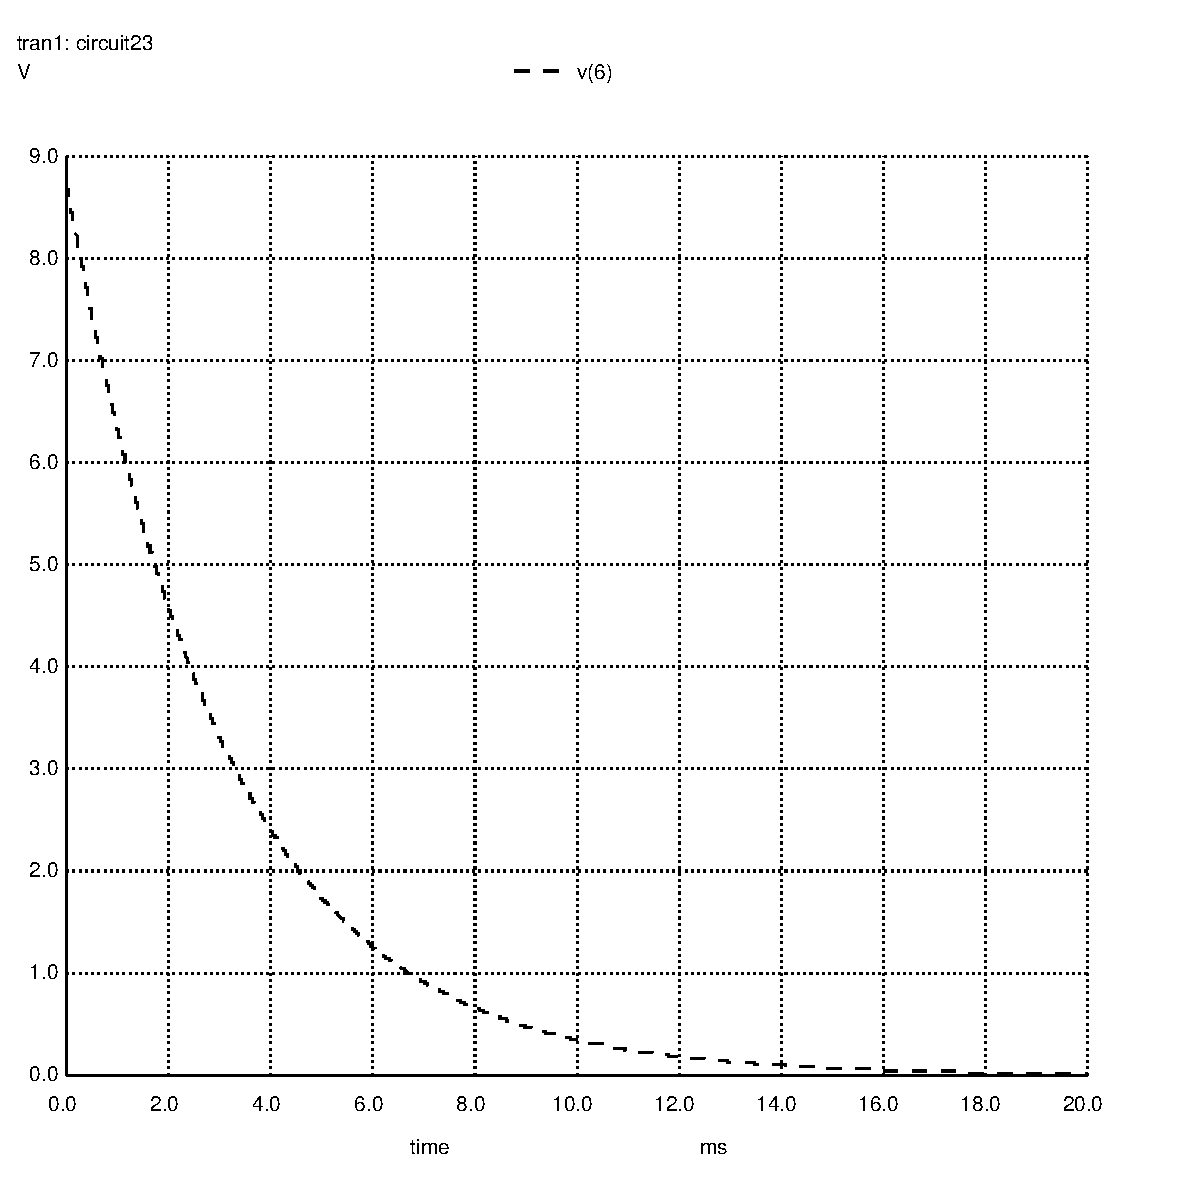
\includegraphics[width=0.8\linewidth]{naturalsolution.eps}
\caption{Plot of v6n(t) in the interval [0, 20]ms.}
\label{fig:plotA(4)}
\end{figure}

In step (4), the forced solution v6f(t) was determined for f=1KHz and for t in the interval [0,20]ms. Moreover, the capacitance was replaced by the impedance, 'Z', and Vs was considered equal to one, representing its amplitude.
The system of equations derived to compute the complex amplitudes is given by: 

\begin{equation}
  V1 = 1
\end{equation}

\begin{equation}
  V1\frac{1}{R1} -V2(\frac{1}{R1}+\frac{1}{R2}+\frac{1}{R3})  + V3\frac{1}{R2} + V5\frac{1}{R3} = 0
\end{equation}

\begin{equation}
  -V2(Kb+\frac{1}{R2}) +V3\frac{1}{R2} + V5Kb = 0
\end{equation}

\begin{equation}
  V5 + V7(\frac{Kd}{R6}) - V8= 0
\end{equation}

\begin{equation}
  -V7(\frac{1}{R6}+\frac{1}{R7}) + V8\frac{1}{R7}= 0
\end{equation}

\begin{equation}
  V2(\frac{1}{R3})  - V5(\frac{1}{R3} +\frac{1}{R5} +\frac{1}{R4}) + V6(\frac{1}{R5} + \frac{1}{Zc}) + V7\frac{1}{R7} - V8(frac{1}{R7} + \frac{1}{Zc}) = 0
\end{equation}

\begin{equation}
   V2(Kb)  - V5(\frac{1}{R5} +Kb) + V6(\frac{1}{R5} + \frac{1}{Zc}) - V8\frac{1}{Zc} = 0
\end{equation}

The complex amplitudes in the nodes are shown in Table~\ref{tab:TA4}.

\begin{table}[h]
  \centering
  \begin{tabular}{|l|r|}
    \hline    
    {\bf Nodes} & {\bf Complex Amplitudes} \\ \hline
    |v1| & 1.000000 \\ \hline
|v2| & 0.960156 \\ \hline
|v3| & 0.878462 \\ \hline
|v4| & 0.000000 \\ \hline
|v5| & 0.965620 \\ \hline
|v6| & -0.609606 \\ \hline
|v7| & -0.408190 \\ \hline
|v8| & -0.613836 \\ \hline
  \end{tabular}
  \caption{Complex amplitudes in the nodes, expressed in Volt.}
  \label{tab:TA4}
\end{table}

Then, in step (5), we determined the final total solution v6(t) by converting the phasors to real time functions for f=1KHz, and superimposing the natural and forced solutions, just like it was asked by the professor. In Figure~\ref{fig:plotA(5)} are plotted both vs(t) and v6(t) in the interval [-5, 20]ms.

\begin{figure}[h] \centering
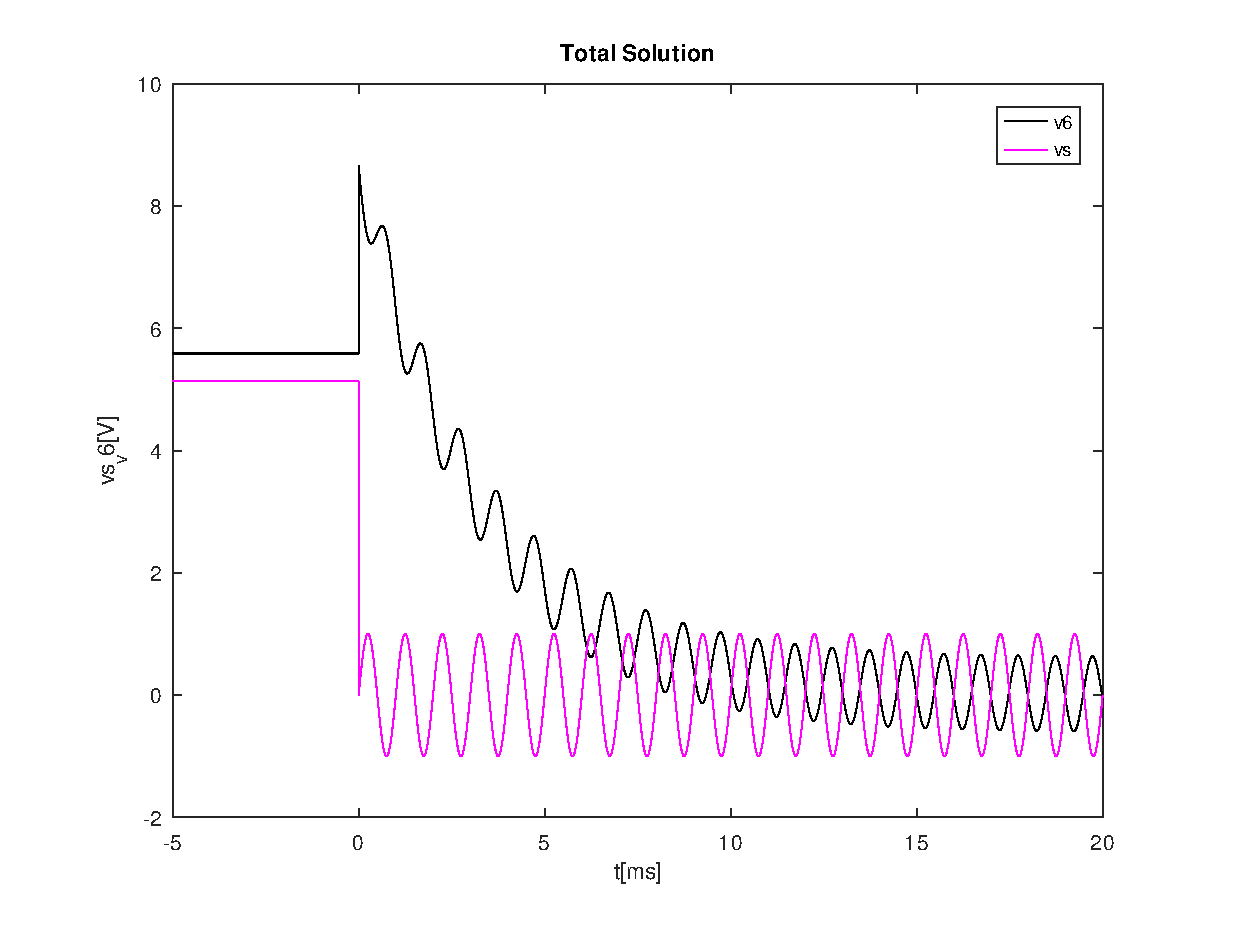
\includegraphics[width=0.8\linewidth]{TotalSolution.eps}
\caption{Plot of v6(t) and vs(t) in the interval [-5, 20]ms.}
\label{fig:plotA(5)}
\end{figure}

Finally, in step (6) of our theoretical analysis, we attempted to figure out the frequency response of the circuit, computing the magnitude and the phase changes with the frequency of both the source voltage, the voltage across the capacitor and the voltage in node 6, and then proceding to plot them.
To do so, we have octave solving the following equations:

\begin{equation}
  V1(\frac{1}{R1}) - V2(\frac{1}{R1}+\frac{1}{R2}+\frac{1}{R3})  + V3\frac{1}{R2} + V5\frac{1}{R3} = 0
\end{equation}

\begin{equation}
  V1 = 1
\end{equation}

\begin{equation}
  V2(\frac{1}{R3}) - V5(\frac{1}{R3}+\frac{1}{R4}+\frac{1}{R5})  + V6(\frac{1}{R5} + \frac{1}{Zc} ) + V7\frac{1}{R7} - V8(\frac{1}{R7} + \frac{1}{Zc} = 0
\end{equation}

\begin{equation}
  V2(Kb+\frac{1}{R2}) -V3\frac{1}{R2} - V5Kb = 0
\end{equation}

\begin{equation}
  V2Kb  + V6(\frac{1}{R5}+\frac{1}{Zc}) - V5(\frac{1}{R5} + Kb) - V8\frac{1}{Zc} = 0
\end{equation}

\begin{equation}
  V7(\frac{1}{R6}+\frac{1}{R7}) - V8\frac{1}{R7}= 0
\end{equation}

\begin{equation}
  V5 + V7\frac{Kd}{R6} - V8 = 0
\end{equation}

Where Zc = 1/(j*w*C) and w=2*$\pi$*f.

The source's magnitude and phase do not hinge on the frequency values, so they are expected to remain constant as it is verified in Figure~\ref{fig:plotA(61)} and Figure~\ref{fig:plotA(62)}.

\begin{figure}[h] \centering
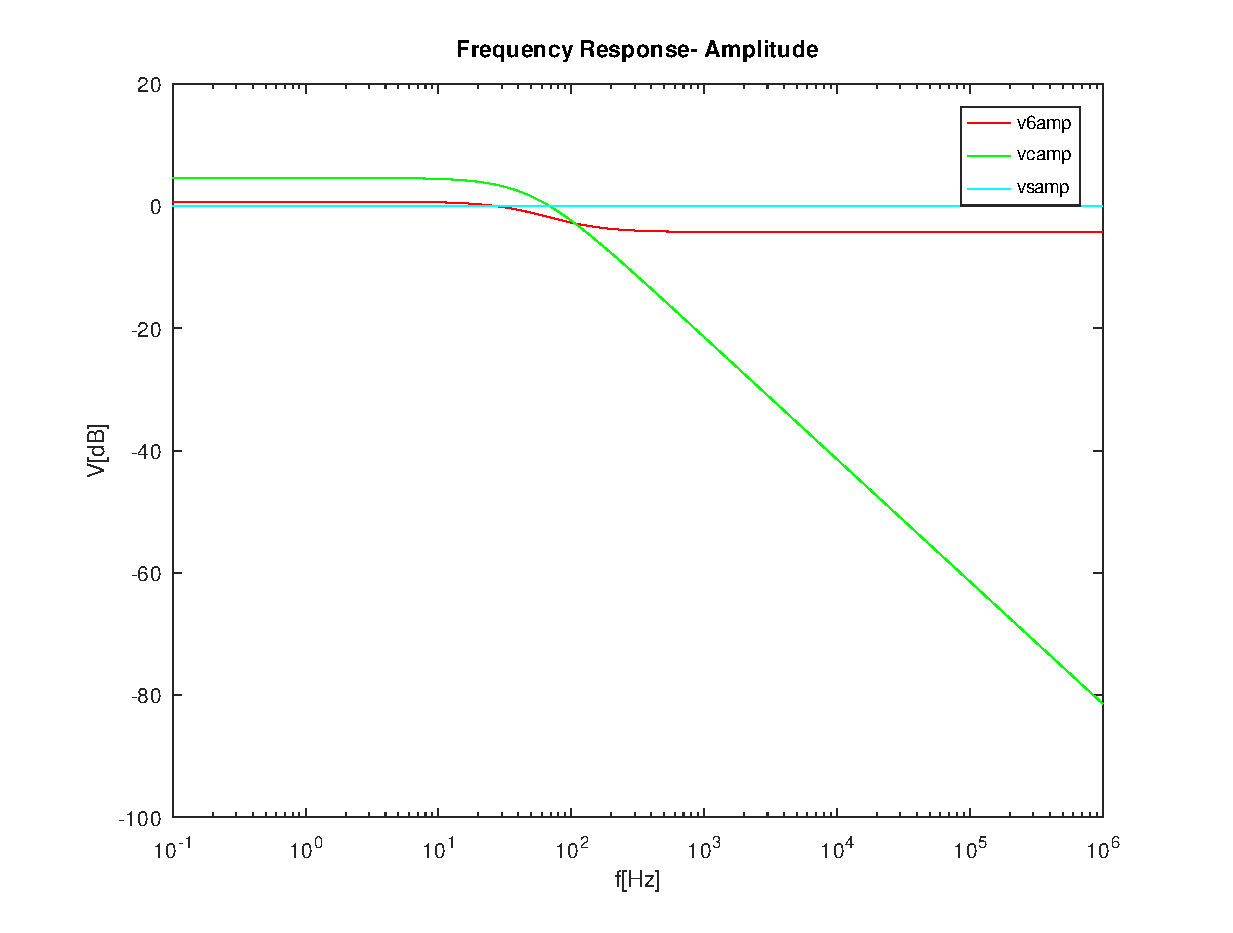
\includegraphics[width=0.6\linewidth]{FrequencyResponseAmplitude.eps}
\caption{Plot of amplitude frequency response (for vs(f), vc(f) and v6(f)) in the interval [0.1, 1M]Hz.}
\label{fig:plotA(61)}
\end{figure}

\begin{figure}[h] \centering
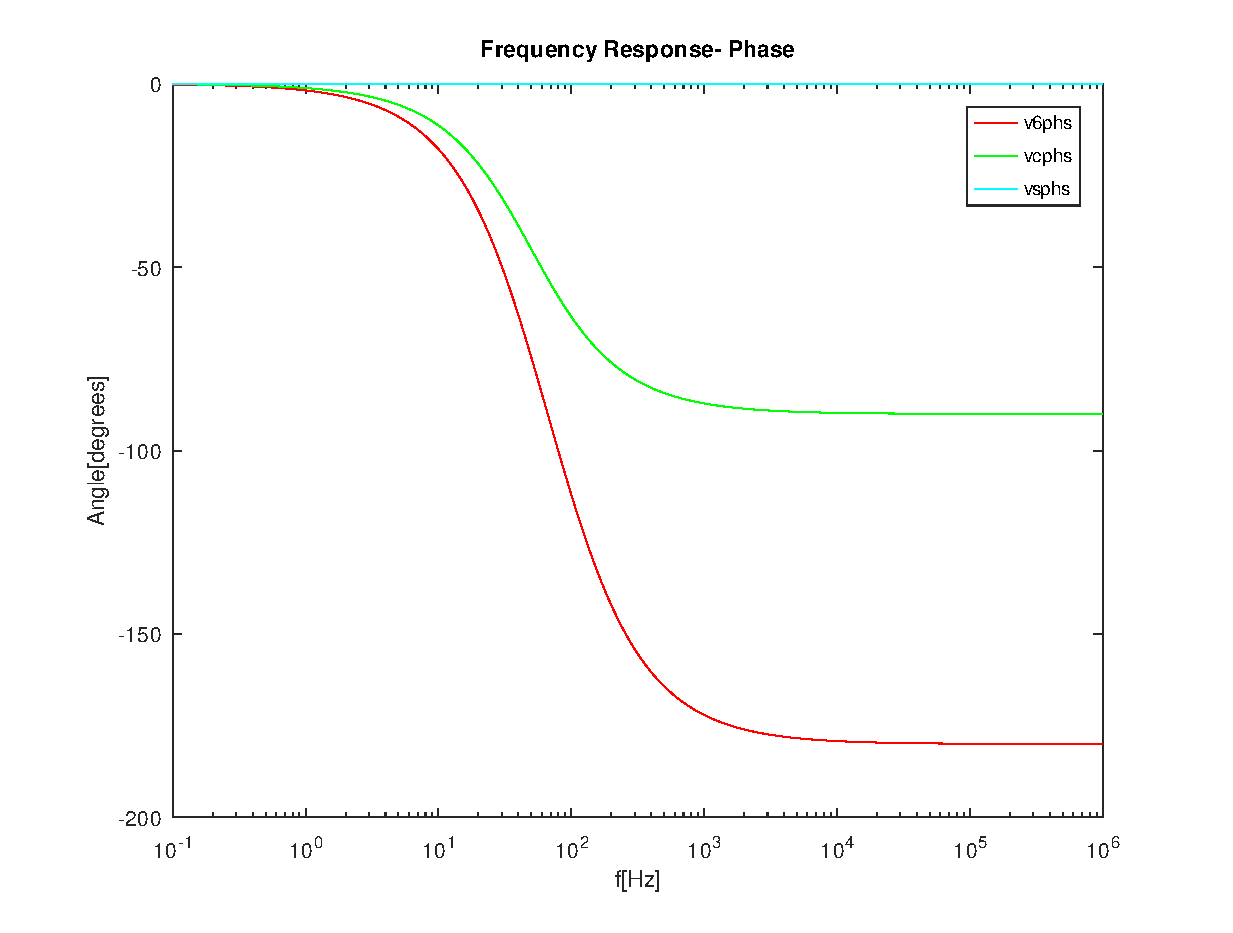
\includegraphics[width=0.6\linewidth]{FrequencyResponsePhase.eps}
\caption{Plot of phase response (for vs(f), vc(f) and v6(f)) in the interval [0.1, 1M]Hz.}
\label{fig:plotA(62)}
\end{figure}

At low frequencies, the capacitor is able to charge up until its voltage reaches a value close to the input's. Therefore, the potential difference across the capacitor rises to a significant value. The voltage at node 6 and the voltage in the capacitor are showcased in the Figure~\ref{fig:plotA(61)} When this is the case, the current flow to the capacitor plummets to a value close to zero, meaning that the circuit will behave as an open circuit. By the same reasoning, it can be concluded that the phase will also behave in the same way as the input's, without showing great disparity, as is shown in Figure~\ref{fig:plotA(62)}. 
On the other hand, as the frequency values increase, the circuit will begin to act as a short circuit (shunt). At this point, the voltage drop in the capacitor's terminals is almost null. When converting the amplitude values from V into dB, a number much smaller than 1 turns into a magnitude that is negative despite having a great absolute value. This is the reason that leads to the visible slump corresponding to vc in Figure~\ref{fig:plotA(61)}. Due to the huge frequency of the source, the phase difference of vc and v6 also become notable, as shown in Figure~\ref{fig:plotA(62)}.

